\documentclass[xcolor=dvipsnames]{beamer}
\usetheme{metropolis}
\usefonttheme{professionalfonts}
\usepackage{algorithm, algpseudocode}
\usepackage{tikz}
\usetikzlibrary{shapes, fit, calc}
\usepackage{fontawesome}
\usepackage{xcolor}
\usepackage{tabularx}
\usepackage{pgfplots}
\usepackage{pgfplotstable}
\pgfplotsset{compat=1.7}
\usepackage{graphicx}
\graphicspath{ {./res/} }

%Information to be included in the title page:
\title{Contention and Space Management in B-Trees}
\author{Christoph Rotte}
\date{22 November 2021}
\institute{Seminar: Implementation Techniques for Main Memory Database Systems}

\begin{document}
	
\frame{\titlepage}

% 
\begin{frame}
	\frametitle{Contention and Space Management in B-Trees}
	
	\begin{itemize}
		\item Paper by \textbf{Adnan Alhomssi} and \textbf{Viktor Leis} (2021)
		\item Two techniques counteracting \textbf{contention} and \textbf{page evictions} (in B-Tree environments)
	\end{itemize}
	
\end{frame}
%
\begin{frame}
\frametitle{B-Trees in Databases}

\begin{center}
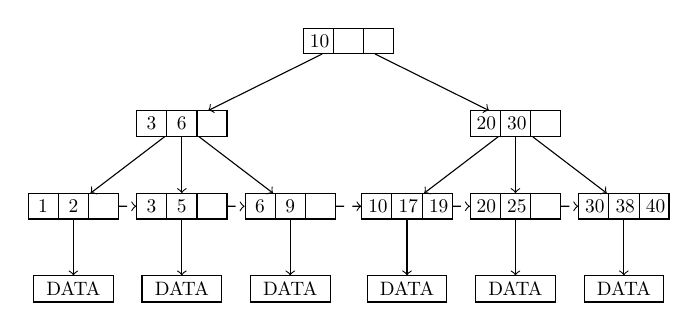
\begin{tikzpicture}[scale=0.7, transform shape]
	\tikzstyle{treenode}=[
	draw,
	rectangle split,
	rectangle split horizontal,
	rectangle split parts=3,
	text width=2ex,
	text centered
	]
	\tikzstyle{datanode}=[
	draw,
	rectangle,
	text centered,
	text width=8ex
	]
	\tikzstyle{level 1}=[sibling distance=40ex]
	\tikzstyle{level 2}=[sibling distance=13ex]
	\node[treenode] {10 \nodepart{two} \nodepart{three}} [->]
	child {node[treenode] {3 \nodepart{two} 6 \nodepart{three}}
		child {node[treenode] (A) {1 \nodepart{two} 2 \nodepart{three}}
			child {node[datanode] {DATA}}
		}
		child {node[treenode] (B) {3 \nodepart{two} 5 \nodepart{three}}
			child {node[datanode] {DATA}}
		}
		child {node[treenode] (C) {6 \nodepart{two} 9 \nodepart{three}}
			child {node[datanode] {DATA}}
		}    
	} 
	child {node[treenode] {20 \nodepart{two} 30 \nodepart{three}}
		child {node[treenode] (D) {10 \nodepart{two} 17 \nodepart{three} 19}
			child {node[datanode] {DATA}}
		}
		child {node[treenode] (E) {20 \nodepart{two} 25 \nodepart{three}}
			child {node[datanode] {DATA}}
		}  
		child {node[treenode] (F) {30 \nodepart{two} 38 \nodepart{three} 40}
			child {node[datanode] {DATA}}
		}     
	};
	\path [->, dashed] (A) edge [right] (B);
	\path [->, dashed] (B) edge [right] (C);
	\path [->, dashed] (C) edge [right] (D);
	\path [->, dashed] (D) edge [right] (E);
	\path [->, dashed] (E) edge [right] (F);
\end{tikzpicture}
\end{center}
\end{frame}
%

\begin{frame}
\frametitle{B-Trees in Databases}

\begin{center}
	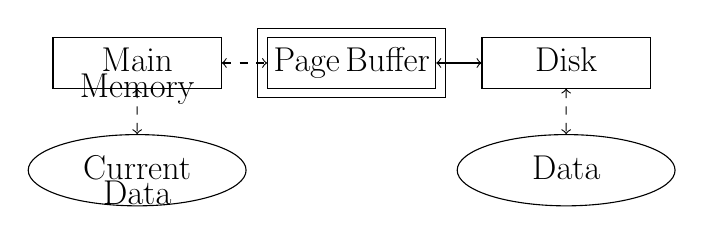
\begin{tikzpicture}[scale=0.6, transform shape]
		\tikzstyle{box}=[
		draw,
		rectangle,
		text centered,
		text depth=1.5ex,
		text height=4ex,
		text width=22ex]
		\tikzstyle{round}=[
		draw,
		ellipse,
		text centered,
		text depth=1.5ex,
		text height=4ex,
		text width=20ex]
		\node[box] (B) {\huge Page Buffer};
		\node[box, left of=B, node distance=30ex] (MM) {\huge Main Memory};
		\node[box, right of=B, node distance=30ex] (D) {\huge Disk};
		\node[round, below of=MM, node distance=15ex] (MM_C) {\huge Current Data};
		\node[round, below of=D, node distance=15ex] (D_C) {\huge Data};
		%
		\path [<->, dashed] (MM) edge [right] (B);
		\path [<->] (B) edge [right] (D);
		\path [<->, dashed] (MM) edge [below] (MM_C);
		\path [<->, dashed] (D) edge [below] (D_C);
		%
		\node[draw=black, fit=(B)] {};
	\end{tikzpicture}
\end{center}

\end{frame}
%
\begin{frame}
\frametitle{B-Trees in Databases}
	
	\begin{center}
		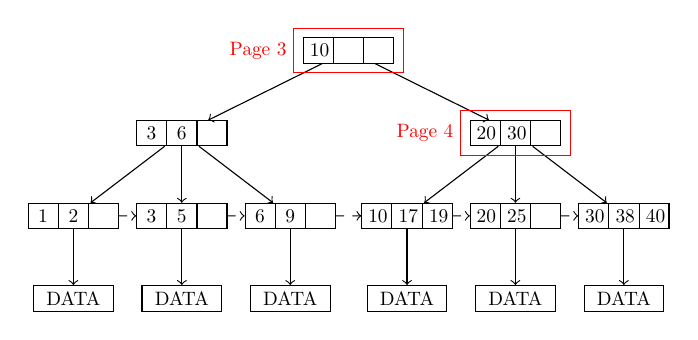
\begin{tikzpicture}[scale=0.7, transform shape]
			\tikzstyle{treenode}=[
			draw,
			rectangle split,
			rectangle split horizontal,
			rectangle split parts=3,
			text width=2ex,
			text centered
			]
			\tikzstyle{datanode}=[
			draw,
			rectangle,
			text centered,
			text width=8ex
			]
			\tikzstyle{level 1}=[sibling distance=40ex]
			\tikzstyle{level 2}=[sibling distance=13ex]
			\node[treenode] (ROOT) {10 \nodepart{two} \nodepart{three}} [->]
			child {node[treenode] (LEFT) {3 \nodepart{two} 6 \nodepart{three}}
				child {node[treenode] (A) {1 \nodepart{two} 2 \nodepart{three}}
					child {node[datanode] {DATA}}
				}
				child {node[treenode] (B) {3 \nodepart{two} 5 \nodepart{three}}
					child {node[datanode] {DATA}}
				}
				child {node[treenode] (C) {6 \nodepart{two} 9 \nodepart{three}}
					child {node[datanode] {DATA}}
				}    
			} 
			child {node[treenode] (RIGHT) {20 \nodepart{two} 30 \nodepart{three}}
				child {node[treenode] (D) {10 \nodepart{two} 17 \nodepart{three} 19}
					child {node[datanode] {DATA}}
				}
				child {node[treenode] (E) {20 \nodepart{two} 25 \nodepart{three}}
					child {node[datanode] {DATA}}
				}  
				child {node[treenode] (F) {30 \nodepart{two} 38 \nodepart{three} 40}
					child {node[datanode] {DATA}}
				}     
			};
			\path [->, dashed] (A) edge [right] (B);
			\path [->, dashed] (B) edge [right] (C);
			\path [->, dashed] (C) edge [right] (D);
			\path [->, dashed] (D) edge [right] (E);
			\path [->, dashed] (E) edge [right] (F);
			%
			\node[draw=red, fit=(ROOT), label=left:{\color{red} Page 3}, text=red] {};
			\node[draw=red, fit=(RIGHT), label=left:{\color{red} Page 4}, text=red] {};
		\end{tikzpicture}
	\end{center}
\end{frame}
% 
\begin{frame}
	\frametitle{B-Trees in Databases}
	
	\begin{center}
		\begin{tikzpicture}[scale=0.7, transform shape]
			\tikzstyle{treenode}=[
			draw,
			rectangle split,
			rectangle split horizontal,
			rectangle split parts=3,
			text width=2ex,
			text centered
			]
			\tikzstyle{datanode}=[
			draw,
			rectangle,
			text centered,
			text width=8ex
			]
			\tikzstyle{level 1}=[sibling distance=40ex]
			\tikzstyle{level 2}=[sibling distance=13ex]
			\node[treenode] (ROOT) {10 \nodepart{two} \nodepart{three}} [->]
			child {node[treenode] (LEFT) {3 \nodepart{two} 6 \nodepart{three}}
				child {node[treenode] (A) {1 \nodepart{two} 2 \nodepart{three}}
					child {node[datanode] {DATA}}
				}
				child {node[treenode] (B) {3 \nodepart{two} 5 \nodepart{three}}
					child {node[datanode] {DATA}}
				}
				child {node[treenode] (C) {6 \nodepart{two} 9 \nodepart{three}}
					child {node[datanode] {DATA}}
				}    
			} 
			child {node[treenode] (RIGHT) {20 \nodepart{two} 30 \nodepart{three}}
				child {node[treenode] (D) {10 \nodepart{two} 17 \nodepart{three} 19}
					child {node[datanode] {DATA}}
				}
				child {node[treenode] (E) {20 \nodepart{two} 25 \nodepart{three}}
					child {node[datanode] {DATA}}
				}  
				child {node[treenode] (F) {30 \nodepart{two} 38 \nodepart{three} 40}
					child {node[datanode] {DATA}}
				}     
			};
			\path [->, dashed] (A) edge [right] (B);
			\path [->, dashed] (B) edge [right] (C);
			\path [->, dashed] (C) edge [right] (D);
			\path [->, dashed] (D) edge [right] (E);
			\path [->, dashed] (E) edge [right] (F);
			%
			\node[draw=red, fit=(ROOT), label=left:{\color{red} \faLock { (r/w) Page 3}}, text=red] {};
			\node[draw=red, fit=(RIGHT), label=left:{\color{red} \faLock { (r/w) Page 4}}, text=red] {};
		\end{tikzpicture}
	\end{center}
\end{frame}
% 
\begin{frame}
	\frametitle{Node Contention}
	
	\begin{center}
		\begin{tikzpicture}[scale=1.2, transform shape]
			\tikzstyle{thread} = [
			draw,
			ellipse,
			text centered,
			text width=8ex
			]
			\tikzstyle{treenode}=[
			draw,
			rectangle split,
			rectangle split horizontal,
			rectangle split parts=3,
			text width=2ex,
			text centered
			]
			\tikzstyle{datanode}=[
			draw,
			rectangle,
			text centered,
			text width=30ex
			]
			\node[thread] (T1) {Thread 1};
			\node[thread, right of=T1, node distance=15ex] (T2) {Thread 2};
			\coordinate (CENTER) at ($(T1)!0.5!(T2)$);
			
			\node[treenode, below of=CENTER, node distance=10ex] (F) 
				{30 \nodepart{two} 38 \nodepart{three} 40} [->]
				child {node[datanode] {DATA}};
			
			\path [->, color=blue, dashed] (T1) edge node [midway, label=left:{\footnotesize update: 30}] {} (F);
			\path [->, color=blue, dashed] (T2) edge node [midway, label=right:{\footnotesize update: 38}] {} (F);
			%
			\node[draw=red, fit=(F), label=left:{\color{red} \scriptsize \faLock { (r/w)}}, text=red] {};
		\end{tikzpicture}
	\end{center}
\end{frame}
% 

\begin{frame}
\frametitle{Contention Split}

\begin{algorithmic}[1]
	
	\small
	
	\Procedure{post\_update }{$page, update\_index, waited$}
	
	\State $last\_update\leftarrow page.last\_index$
	\State $r\leftarrow random(0.0, 1.0)$
	\If{$\textcolor{red}{r < sample\_prob}$}
	\State \colorbox{yellow}{Update $update\_count, last\_index, wait\_count$ on $page$}
	\EndIf
	
	\If{$\textcolor{red}{r < period\_prob}$} \textcolor{gray}{{} \# $period\_prob < sample\_prob$}
	\If{$page.wait\_times \approx page.update\_times$}
	\State \colorbox{yellow}{Split $page.node$ at mid($update\_index$, $last\_update$)}
	\State Reset $update\_count, last\_index, wait\_count$ on $page$ 
	\EndIf
	\EndIf
	
	\EndProcedure
\end{algorithmic} 
\end{frame}
%
\begin{frame}
	\frametitle{Contention Split}
	
	\begin{center}
		\begin{tikzpicture}[scale=1.2, transform shape]
			\tikzstyle{thread} = [
			draw,
			ellipse,
			text centered,
			text width=8ex
			]
			\tikzstyle{treenode}=[
			draw,
			rectangle split,
			rectangle split horizontal,
			rectangle split parts=3,
			text width=2ex,
			text centered
			]
			\tikzstyle{datanode}=[
			draw,
			rectangle,
			text centered,
			text width=30ex
			]
			\node[thread] (T1) {Thread 1};
			\node[thread, right of=T1, node distance=15ex] (T2) {Thread 2};
			\coordinate (CENTER) at ($(T1)!0.5!(T2)$);
			
			\node[treenode, below of=CENTER, node distance=10ex] (F) 
			{30 \nodepart{two} 38 \nodepart{three} 40} [->]
			child {node[datanode] {DATA}};
			
			\path [->, color=red, dashed] (T1) edge node [midway, label=left:{\footnotesize updating: 30}] {} (F);
			\path [->, color=blue, dashed] (T2) edge node [midway, label=right:{\footnotesize waiting: 38}] {} (F);
			%
			\node[draw=red, fit=(F), label=left:{\color{red} \scriptsize \faLock {}}, text=red] {};
		\end{tikzpicture}
	\end{center}
\end{frame}
%
\begin{frame}
	\frametitle{Contention Split}
	
	\begin{center}
		\begin{tikzpicture}[scale=1.2, transform shape]
			\tikzstyle{thread} = [
			draw,
			ellipse,
			text centered,
			text width=8ex
			]
			\tikzstyle{treenode}=[
			draw,
			rectangle split,
			rectangle split horizontal,
			rectangle split parts=3,
			text width=2ex,
			text centered
			]
			\tikzstyle{datanode}=[
			draw,
			rectangle,
			text centered,
			text width=30ex
			]
			\node[thread] (T1) {Thread 1};
			\node[thread, right of=T1, node distance=15ex] (T2) {Thread 2};
			
			\node[treenode, below of=T1, node distance=10ex] (F1) 
			{30 \nodepart{two} \nodepart{three}};
			\node[treenode, below of=T2, node distance=10ex] (F2) 
			{38 \nodepart{two} 40 \nodepart{three}};
			
			\coordinate (CENTER) at ($(F1)!0.5!(F2)$);
			\node[datanode, below of=CENTER, node distance=10ex] (D) {DATA};
			
			\path [->, color=red, dashed] (T1) edge node [midway, label=left:{\footnotesize updating: 30}] {} (F1);
			\path [->, color=red, dashed] (T2) edge node [midway, label=right:{\footnotesize updating: 38}] {} (F2);
			
			\path [->] (F1) edge (D);
			\path [->] (F2) edge (D);
			%
			\node[draw=red, fit=(F1), label=left:{\color{red} \scriptsize \faLock {}}, text=red] {};
			\node[draw=red, fit=(F2), label=left:{\color{red} \scriptsize \faLock {}}, text=red] {};
		\end{tikzpicture}
	\end{center}
\end{frame}
%
\begin{frame}
	\frametitle{Page Evictions}
	
	\begin{center}
		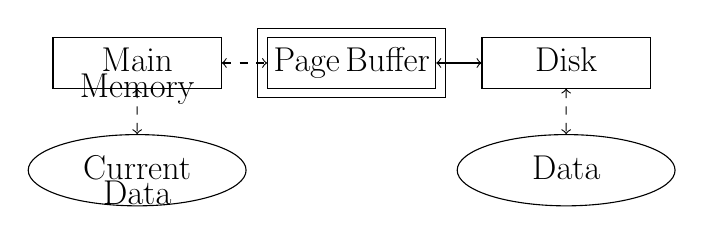
\begin{tikzpicture}[scale=0.6, transform shape]
			\tikzstyle{box}=[
			draw,
			rectangle,
			text centered,
			text depth=1.5ex,
			text height=4ex,
			text width=22ex]
			\tikzstyle{round}=[
			draw,
			ellipse,
			text centered,
			text depth=1.5ex,
			text height=4ex,
			text width=20ex]
			\node[box] (B) {\huge Page Buffer};
			\node[box, left of=B, node distance=30ex] (MM) {\huge Main Memory};
			\node[box, right of=B, node distance=30ex] (D) {\huge Disk};
			\node[round, below of=MM, node distance=15ex] (MM_C) {\huge Current Data};
			\node[round, below of=D, node distance=15ex] (D_C) {\huge Data};
			%
			\path [<->, dashed] (MM) edge [right] (B);
			\path [<->] (B) edge [right] (D);
			\path [<->, dashed] (MM) edge [below] (MM_C);
			\path [<->, dashed] (D) edge [below] (D_C);
			%
			\node[draw=black, fit=(B)] {};
		\end{tikzpicture}
	\end{center}
	
\end{frame}
%
\begin{frame}
	\frametitle{X-Merge}
	
	\begin{algorithmic}[1]
		
		\footnotesize
		
		\Procedure{pre\_eviction }{$requested\_id$}
		\State \colorbox{yellow}{$node\leftarrow random\_inner\_node()$}
		\If{not $is\_qualified(node)$}
		\State return
		\EndIf
		
		\State \colorbox{yellow}{$start\_index\leftarrow random\_index(node)$}
		\State $i\leftarrow 0$
		\State $space\leftarrow 0$
		
		\While{$i < \textcolor{red}{max\_nodes}$ and $space < \textcolor{red}{node\_size}$}
			\State \colorbox{yellow}{$space\leftarrow space + node.child[start\_index + i].free\_space$}
			\State $i\leftarrow i + 1$
		\EndWhile
		
		\If{$space >= \textcolor{red}{node\_size}$}
		\State \colorbox{yellow}{$merge\_children(start\_index, start\_index + i)$}
		\State $load\_page(node.child[start\_index], requested\_id)$
		\EndIf

		\EndProcedure
	\end{algorithmic} 
\end{frame}

% 
\begin{frame}
	\frametitle{X-Merge}
	
	\begin{center}
		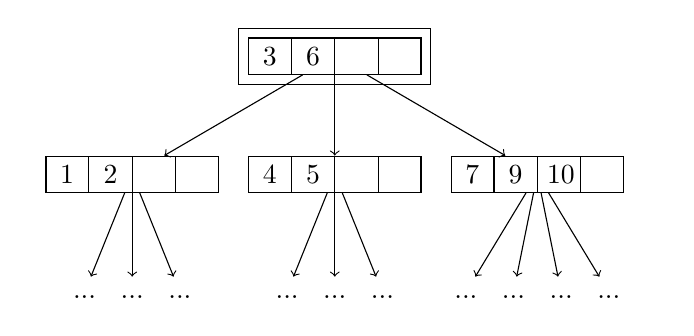
\begin{tikzpicture}[scale=1, transform shape]
			\tikzstyle{treenode}=[
			draw,
			rectangle split,
			rectangle split horizontal,
			rectangle split parts=4,
			text width=2ex,
			text centered
			]
			\tikzstyle{datanode}=[
			rectangle,
			text centered,
			text width=8ex,
			text height=1ex
			]
			\tikzstyle{level 1}=[sibling distance=17ex]
			\tikzstyle{level 2}=[sibling distance=4ex]
			\node[treenode] (LEFT) {3 \nodepart{two} 6 \nodepart{three} \nodepart{four}} [->]
			child {node[treenode] (A) {1 \nodepart{two} 2 \nodepart{three} \nodepart{four}}
				child {node[datanode] {...}}
				child {node[datanode] {...}}
				child {node[datanode] {...}}
			}
			child {node[treenode] (B) {4 \nodepart{two} 5 \nodepart{three} \nodepart{four}}
				child {node[datanode] {...}}
				child {node[datanode] {...}}
				child {node[datanode] {...}}
			}
			child {node[treenode] (C) {7 \nodepart{two} 9 \nodepart{three} 10 \nodepart{four}}
				child {node[datanode] {...}}
				child {node[datanode] {...}}
				child {node[datanode] {...}}
				child {node[datanode] {...}}
			};
			\node[draw=black, fit=(LEFT)] {};
			%\path [->, dashed] (E) edge [right] (F);
			%
			%\node[draw=red, fit=(ROOT), label=left:{\color{red} \faLock { (r/w) Page 3}}, text=red] {};
			%\node[draw=red, fit=(RIGHT), label=left:{\color{red} \faLock { (r/w) Page 4}}, text=red] {};
		\end{tikzpicture}
	\end{center}
\end{frame}

% 
\begin{frame}
	\frametitle{X-Merge}
	
	\begin{center}
		\hspace*{0.5ex}
		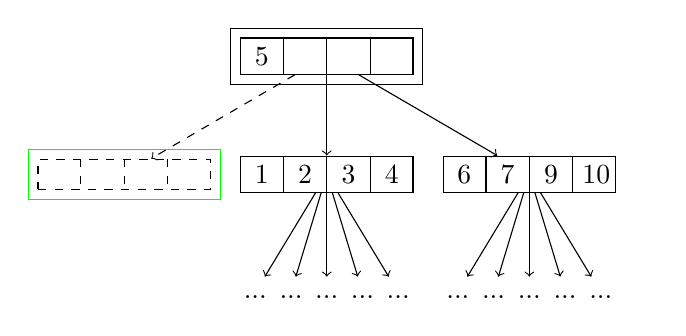
\begin{tikzpicture}[scale=1, transform shape]
			\tikzstyle{treenode}=[
			draw,
			rectangle split,
			rectangle split horizontal,
			rectangle split parts=4,
			text width=2ex,
			text centered
			]
			\tikzstyle{datanode}=[
			rectangle,
			text centered,
			text width=8ex,
			text height=1ex
			]
			\tikzstyle{level 1}=[sibling distance=17ex]
			\tikzstyle{level 2}=[sibling distance=3ex]
			\node[treenode] (LEFT) {5 \nodepart{two} \nodepart{three} \nodepart{four}} [->] 
			child [dashed] {node[treenode] (A) {\phantom{a} \nodepart{two} \nodepart{three} \nodepart{four}}
			}
			child {node[treenode] (B) {1 \nodepart{two} 2 \nodepart{three} 3 \nodepart{four} 4}
				child {node[datanode] {...}}
				child {node[datanode] {...}}
				child {node[datanode] {...}}
				child {node[datanode] {...}}
				child {node[datanode] {...}}
			}
			child {node[treenode] (C) {6 \nodepart{two} 7 \nodepart{three} 9 \nodepart{four} 10}
				child {node[datanode] {...}}
				child {node[datanode] {...}}
				child {node[datanode] {...}}
				child {node[datanode] {...}}
				child {node[datanode] {...}}
			};
			%
			\node[draw=green, fit=(A)] {};
			\node[draw=black, fit=(LEFT)] {};
		\end{tikzpicture}
	\end{center}
\end{frame}
%

\begin{frame}
	\frametitle{Contention Split vs. X-Merge}
	
	\vspace{2ex}
	\begin{table}[!h]
		\centering
		\begin{tabularx}{\textwidth}{XX}
			{
				
				\begin{center}
					\hspace*{-9ex}
					\begin{tikzpicture}[scale=0.7, transform shape]
						\tikzstyle{thread} = [
						draw,
						ellipse,
						text centered,
						text width=8ex
						]
						\tikzstyle{treenode}=[
						draw,
						rectangle split,
						rectangle split horizontal,
						rectangle split parts=3,
						text width=2ex,
						text centered
						]
						\tikzstyle{datanode}=[
						draw,
						rectangle,
						text centered,
						text width=30ex
						]
						\node[thread] (T1) {Thread 1};
						\node[thread, right of=T1, node distance=15ex] (T2) {Thread 2};
						
						\node[treenode, below of=T1, node distance=10ex] (F1) 
						{30 \nodepart{two} \nodepart{three}};
						\node[treenode, below of=T2, node distance=10ex] (F2) 
						{38 \nodepart{two} 40 \nodepart{three}};
						
						\coordinate (CENTER) at ($(F1)!0.5!(F2)$);
						\node[datanode, below of=CENTER, node distance=10ex] (D) {DATA};
						
						\path [->, color=red, dashed] (T1) edge node [midway] {} (F1);
						\path [->, color=red, dashed] (T2) edge node [midway] {} (F2);
						
						\path [->] (F1) edge (D);
						\path [->] (F2) edge (D);
						%
						\node[draw=red, fit=(F1), label=left:{\color{red} \scriptsize \faLock {}}, text=red] {};
						\node[draw=red, fit=(F2), label=left:{\color{red} \scriptsize \faLock {}}, text=red] {};
					\end{tikzpicture}
					
					\vspace*{3ex}
					\hspace*{-9ex}
					\small Contention Split
				\end{center}
				
			} & {
				\vspace{1.35ex}
				\begin{center}
					\hspace*{-6ex}
					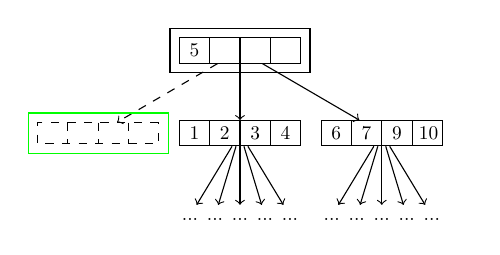
\begin{tikzpicture}[scale=0.7, transform shape]
						\tikzstyle{treenode}=[
						draw,
						rectangle split,
						rectangle split horizontal,
						rectangle split parts=4,
						text width=2ex,
						text centered
						]
						\tikzstyle{datanode}=[
						rectangle,
						text centered,
						text width=8ex,
						text height=1ex
						]
						\tikzstyle{level 1}=[sibling distance=17ex]
						\tikzstyle{level 2}=[sibling distance=3ex]
						\node[treenode] (LEFT) {5 \nodepart{two} \nodepart{three} \nodepart{four}} [->] 
						child [dashed] {node[treenode] (A) {\phantom{a} \nodepart{two} \nodepart{three} \nodepart{four}}
						}
						child {node[treenode] (B) {1 \nodepart{two} 2 \nodepart{three} 3 \nodepart{four} 4}
							child {node[datanode] {...}}
							child {node[datanode] {...}}
							child {node[datanode] {...}}
							child {node[datanode] {...}}
							child {node[datanode] {...}}
						}
						child {node[treenode] (C) {6 \nodepart{two} 7 \nodepart{three} 9 \nodepart{four} 10}
							child {node[datanode] {...}}
							child {node[datanode] {...}}
							child {node[datanode] {...}}
							child {node[datanode] {...}}
							child {node[datanode] {...}}
						};
						%
						\node[draw=green, fit=(A)] {};
						\node[draw=black, fit=(LEFT)] {};
					\end{tikzpicture}
					
					\vspace*{4.75ex}
					\hspace*{-2ex}
					\small X-Merge
				\end{center}
				
			}
		\end{tabularx}
	\end{table}
	
\end{frame}


%

\begin{frame}
\frametitle{Implementation}

\begin{center}
	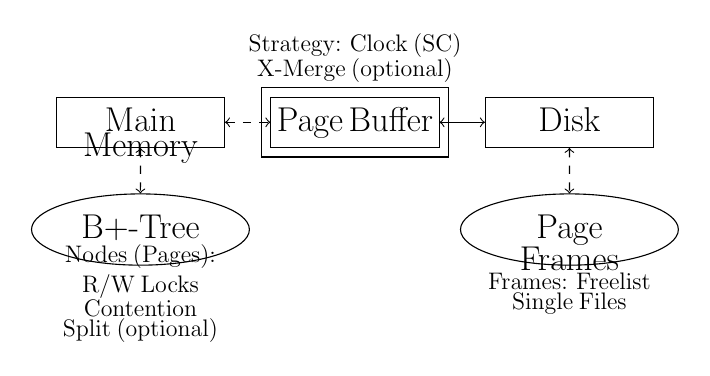
\begin{tikzpicture}[scale=0.6, transform shape]
		\tikzstyle{box}=[
		draw,
		rectangle,
		text centered,
		text depth=1.5ex,
		text height=4ex,
		text width=22ex]
		\tikzstyle{box_empty}=[
		rectangle,
		text centered,
		text width=30ex]
		\tikzstyle{round}=[
		draw,
		ellipse,
		text centered,
		text depth=1.5ex,
		text height=4ex,
		text width=20ex]
		\node[box] (B) {\huge Page Buffer};
		\node[box, left of=B, node distance=30ex] (MM) {\huge Main Memory};
		\node[box, right of=B, node distance=30ex] (D) {\huge Disk};
		\node[round, below of=MM, node distance=15ex] (MM_C) {\huge B+-Tree};
		\node[round, below of=D, node distance=15ex] (D_C) {\huge Page Frames};
		%
		\path [<->, dashed] (MM) edge [right] (B);
		\path [<->] (B) edge [right] (D);
		\path [<->, dashed] (MM) edge [below] (MM_C);
		\path [<->, dashed] (D) edge [below] (D_C);
		%
		\node[draw=black, fit=(B)] {};
		%
		\node[box_empty, above of=B, node distance=9ex] {
			\Large Strategy: Clock (SC)\\X-Merge (optional)};
		%
		\node[box_empty, below of=MM_C, node distance=9ex] {\Large Nodes (Pages): R/W Locks\\Contention Split (optional)};
		\node[box_empty, below of=D_C, node distance=9ex] {\Large Frames: Freelist\\Single Files};
	\end{tikzpicture}
\end{center}

\end{frame}

%

\begin{frame}
\frametitle{Yahoo Cloud Serving Benchmark (YCSB)}
\begin{center}
	\begin{itemize}
		\item \textbf{Different workloads} (with different \textbf{distributions})
		\item Possible operations: insert, delete, read, write, update, scan
		\item Loading phase $\leftrightarrow$ operation phase
		\item Entries: key $\rightarrow$ tuple (10 $\cdot$ 100 bytes)
		\item \textbf{YCSB-cpp}: implementation of YCSB in C++
	\end{itemize}
\end{center}	
\end{frame}

%

\begin{frame}
	\frametitle{Evaluation Setup | Contention Split}
	\begin{center}
		\begin{itemize}
			\item AMD Ryzen 5 2600X (12 threads) | Samsung SSD 860 EVO
			\item Page size: 4 KiB
			\item \textbf{Buffer}: holds all pages in memory
			\item 10M loaded entries + 100M operations
			\item \textbf{Workload}: 20\% reads, 80\% updates
			\item \textbf{Distribution}: Zipfian
			\item \textbf{Parameters}: $sample\_prob$ = 0.5\% | $period\_prob$ = 0.05\%
		\end{itemize}
	\end{center}	
\end{frame}

%

\begin{frame}
\frametitle{Evaluation | Contention Split}
\hspace*{-3ex}
\vspace*{-6ex}
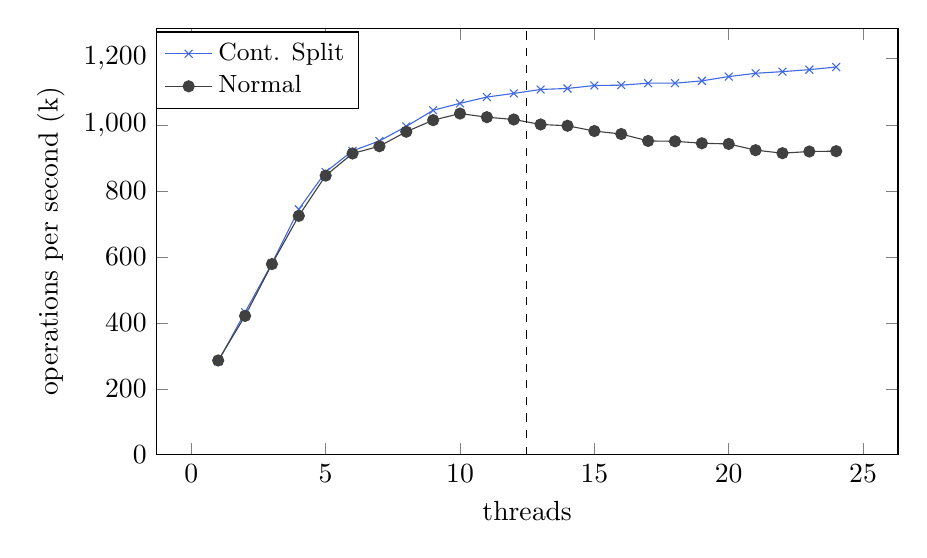
\begin{tikzpicture}
	\begin{axis}[
		xlabel=threads,
		ylabel=operations per second (k),
		width=11cm,height=7cm,
		legend style={at={(-0.001,.902)},anchor=west},
		legend cell align={left},
		ymin=0
		]
		
		\addplot[color=RoyalBlue,mark=x] coordinates {
			(1, 283)
			(2, 432)
			(3, 580)
			(4, 744)
			(5, 857)
			(6, 921)
			(7, 951)
			(8, 995)
			(9, 1044)
			(10, 1065)
			(11, 1084)
			(12, 1095)
			(13, 1107)
			(14, 1110)
			(15, 1119)
			(16, 1120)
			(17, 1126)
			(18, 1126)
			(19, 1133)
			(20, 1146)
			(21, 1156)
			(22, 1161)
			(23, 1167)
			(24, 1175)
		};
		
		\addplot[color=darkgray,mark=*] coordinates {
			(1, 286)
			(2, 421)
			(3, 578)
			(4, 724)
			(5, 846)
			(6, 913)
			(7, 935)
			(8, 979)
			(9, 1014)
			(10, 1034)
			(11, 1023)
			(12, 1016)
			(13, 1001)
			(14, 997)
			(15, 981)
			(16, 972)
			(17, 951)
			(18, 950)
			(19, 944)
			(20, 942)
			(21, 923)
			(22, 914)
			(23, 919)
			(24, 920)
		};
		
		\legend{\small Cont. Split, \small Normal}
	\end{axis}
	\draw [dashed] (4.7, 0) -- (4.7, 5.4);
\end{tikzpicture}

\end{frame}

%

\begin{frame}
	\frametitle{Evaluation Setup | X-Merge}
	\begin{center}
		\begin{itemize}
			\item AMD Ryzen 5 2600X (12 threads) | Samsung SSD 860 EVO
			\item Page size: 4 KiB
			\item \textbf{Buffer}: limited memory 
			\item 10M loaded entries + 100M operations
			\item \textbf{Workload}: 30\% reads, 60\% updates, 10\% inserts
			\item \textbf{Distribution}: Zipfian
			\item \textbf{Parameter}: $max\_nodes$ = 5
			\item Threads: 10
		\end{itemize}
	\end{center}	
\end{frame}

\begin{frame}
	\frametitle{Evaluation | X-Merge}
	\hspace*{-3ex}
	\vspace*{-6ex}
	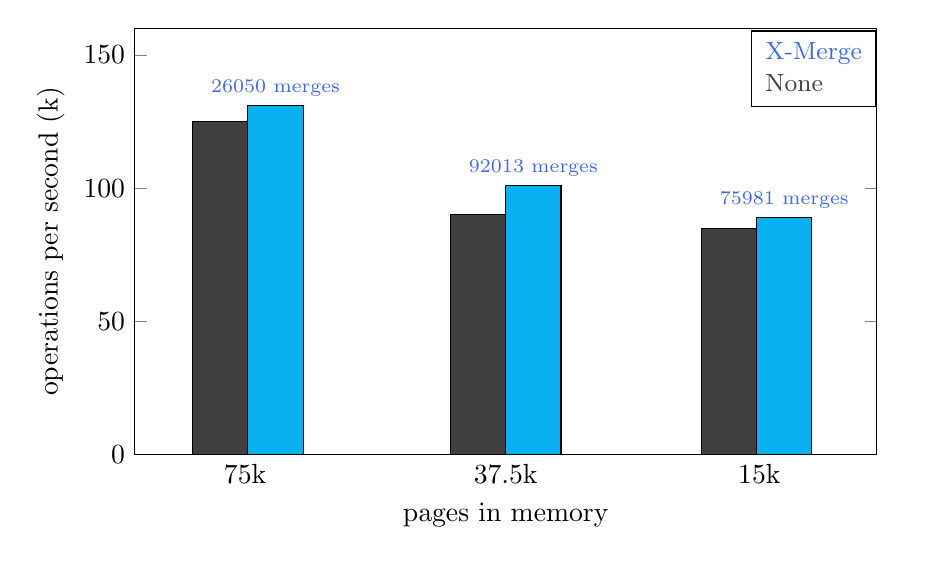
\begin{tikzpicture}
		\begin{axis}[
			xlabel=pages in memory,
			ylabel=operations per second (k),
			width=11cm,height=7cm,
			legend style={at={(1,.905)},anchor=east},
			legend cell align={left},
			ymin=0,
			ymax=160,
			bar width=20pt,
			symbolic x coords={\enspace\quad\qquad75k, 37.5k, 15k\qquad\quad\enspace\enspace},
			xtick={\enspace\quad\qquad75k, 37.5k, 15k\qquad\quad\enspace\enspace},
			xtick style={draw=none},
			legend style={empty legend},
			nodes near coords,
			point meta=explicit symbolic
			]
			
			\addplot[ybar, color=black, fill=ProcessBlue, mark=none, xshift=28.5pt] coordinates {
				(\enspace\quad\qquad75k, 131)[\scriptsize \textcolor{RoyalBlue}{26050 merges}]
			};
			\addplot[ybar, color=black, fill=ProcessBlue, mark=none, xshift=10pt] coordinates {
				(37.5k, 101)[\scriptsize \textcolor{RoyalBlue}{92013 merges}]
			};
			\addplot[ybar, color=black, fill=ProcessBlue, mark=none, xshift=-11pt] coordinates {
				(15k\qquad\quad\enspace\enspace, 89)[\scriptsize \textcolor{RoyalBlue}{75981 merges}]
			};
			
			\addplot[ybar, color=black, fill=darkgray, mark=none, xshift=8.5pt] coordinates {
				(\enspace\quad\qquad75k, 125)
			};
			\addplot[ybar, color=black, fill=darkgray, mark=none, xshift=-10pt] coordinates {
				(37.5k, 90)
			};
			\addplot[ybar, color=black, fill=darkgray, mark=none, xshift=-31pt] coordinates {
				(15k\qquad\quad\enspace\enspace, 85)
			};
			
			\legend{\small \textcolor{RoyalBlue}{X-Merge}, \small \textcolor{darkgray}{None}}
		\end{axis}
	\end{tikzpicture}
	
\end{frame}
%
\begin{frame}
	\frametitle{Evaluation | Combined}
	\hspace*{-3ex}
	\vspace*{-6ex}
	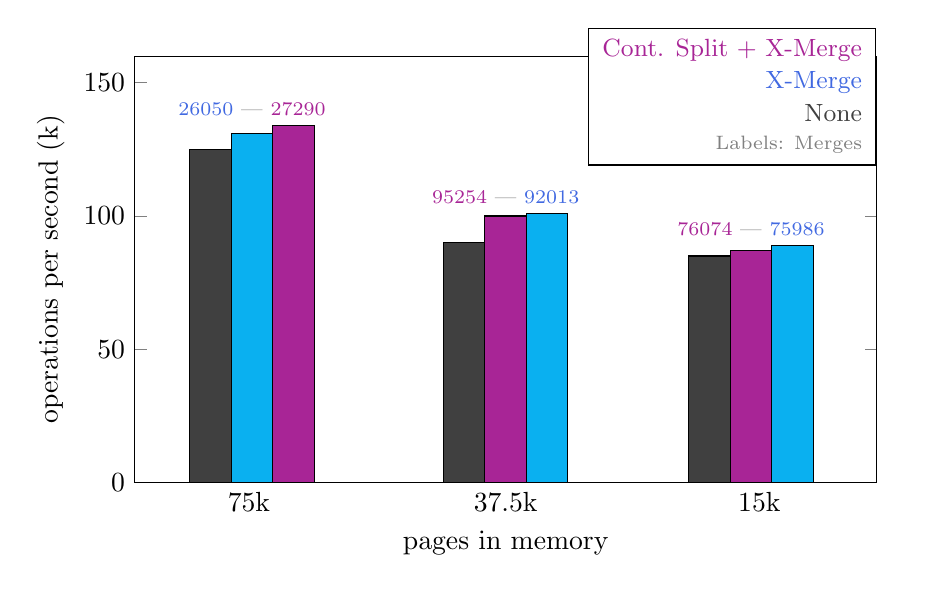
\begin{tikzpicture}
		\begin{axis}[
			xlabel=pages in memory,
			ylabel=operations per second (k),
			width=11cm,height=7cm,
			legend style={at={(1,.905)},anchor=east},
			legend cell align={right},
			ymin=0,
			ymax=160,
			bar width=15pt,
			symbolic x coords={\thickspace\enspace\quad\qquad75k, 37.5k, 15k\qquad\qquad\qquad},
			xtick={\thickspace\enspace\quad\qquad75k, 37.5k, 15k\qquad\qquad\qquad},
			xtick style={draw=none},
			legend style={empty legend},
			nodes near coords,
			point meta=explicit symbolic
			]
			
			\addplot[ybar, color=white, fill=white, mark=none, xshift=20pt] coordinates {
				(\thickspace\enspace\quad\qquad75k, 134)[\scriptsize \textcolor{RoyalBlue}{26050} \textcolor{gray}{|} \textcolor{Mulberry}{27290}]
			};
			\addplot[ybar, color=white, fill=white, mark=none] coordinates {
				(37.5k, 101)[\scriptsize \textcolor{Mulberry}{95254} \textcolor{gray}{|} \textcolor{RoyalBlue}{92013}]
			};
			\addplot[ybar, color=white, fill=white, mark=none, xshift=-23pt] coordinates {
				(15k\qquad\qquad\qquad, 89)[\scriptsize \textcolor{Mulberry}{76074} \textcolor{gray}{|} \textcolor{RoyalBlue}{75986}]
			};
			%
			\addplot[ybar, color=black, fill=Mulberry, mark=none, xshift=35pt] coordinates {
				(\thickspace\enspace\quad\qquad75k, 134)
			};
			\addplot[ybar, color=black, fill=ProcessBlue, mark=none, xshift=15pt] coordinates {
				(37.5k, 101)
			};
			\addplot[ybar, color=black, fill=ProcessBlue, mark=none, xshift=-8pt] coordinates {
				(15k\qquad\qquad\qquad, 89)
			};
			
			
			\addplot[ybar, color=black, fill=ProcessBlue, mark=none, xshift=20pt] coordinates {
				(\thickspace\enspace\quad\qquad75k, 131)
			};
			\addplot[ybar, color=black, fill=Mulberry, mark=none] coordinates {
				(37.5k, 100)
			};
			\addplot[ybar, color=black, fill=Mulberry, mark=none, xshift=-23pt] coordinates {
				(15k\qquad\qquad\qquad, 87)
			};
			
			\addplot[ybar, color=black, fill=darkgray, mark=none, xshift=5pt] coordinates {
				(\thickspace\enspace\quad\qquad75k, 125)
			};
			\addplot[ybar, color=black, fill=darkgray, mark=none, xshift=-15pt] coordinates {
				(37.5k, 90)
			};
			\addplot[ybar, color=black, fill=darkgray, mark=none, xshift=-38pt] coordinates {
				(15k\qquad\qquad\qquad, 85)
			};
			
			\legend{\small \textcolor{Mulberry}{Cont. Split + X-Merge}, 
				\small \textcolor{RoyalBlue}{X-Merge},
				\small \textcolor{darkgray}{None},
				\scriptsize \textcolor{gray}{Labels: Merges}}
		\end{axis}
	\end{tikzpicture}
	
\end{frame}

%

\begin{frame}
\frametitle{Contention Split and X-Merge in Leanstore}
	
\begin{figure}
	\vspace*{2ex}
	\centering
	\fcolorbox{gray}{white}{\includegraphics[scale=1.1]{leanstore}}
	
	Leanstore: TPC-C | buffer=240GiB | workers=120 \scriptsize (Alhomssi \& Leis)
\end{figure}
	
\end{frame}

%

\begin{frame}
	\frametitle{Conclusion}
	
	\vspace{2ex}
	\begin{table}[!h]
		\centering
		\begin{tabularx}{\textwidth}{XX}
			{
				
				\begin{center}
					\hspace*{-9ex}
					\begin{tikzpicture}[scale=0.7, transform shape]
						\tikzstyle{thread} = [
						draw,
						ellipse,
						text centered,
						text width=8ex
						]
						\tikzstyle{treenode}=[
						draw,
						rectangle split,
						rectangle split horizontal,
						rectangle split parts=3,
						text width=2ex,
						text centered
						]
						\tikzstyle{datanode}=[
						draw,
						rectangle,
						text centered,
						text width=30ex
						]
						\node[thread] (T1) {Thread 1};
						\node[thread, right of=T1, node distance=15ex] (T2) {Thread 2};
						
						\node[treenode, below of=T1, node distance=10ex] (F1) 
						{30 \nodepart{two} \nodepart{three}};
						\node[treenode, below of=T2, node distance=10ex] (F2) 
						{38 \nodepart{two} 40 \nodepart{three}};
						
						\coordinate (CENTER) at ($(F1)!0.5!(F2)$);
						\node[datanode, below of=CENTER, node distance=10ex] (D) {DATA};
						
						\path [->, color=red, dashed] (T1) edge node [midway] {} (F1);
						\path [->, color=red, dashed] (T2) edge node [midway] {} (F2);
						
						\path [->] (F1) edge (D);
						\path [->] (F2) edge (D);
						%
						\node[draw=red, fit=(F1), label=left:{\color{red} \scriptsize \faLock {}}, text=red] {};
						\node[draw=red, fit=(F2), label=left:{\color{red} \scriptsize \faLock {}}, text=red] {};
					\end{tikzpicture}
				
					\vspace*{3ex}
					\hspace*{-9ex}
					\small Contention Split
				\end{center}
				
			} & {
				\vspace{1.35ex}
				\begin{center}
					\hspace*{-6ex}
					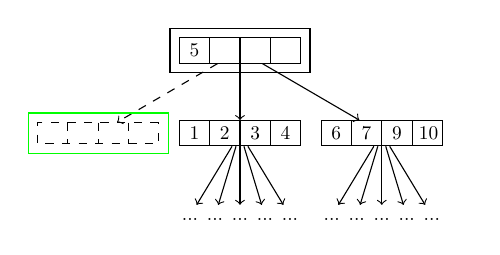
\begin{tikzpicture}[scale=0.7, transform shape]
						\tikzstyle{treenode}=[
						draw,
						rectangle split,
						rectangle split horizontal,
						rectangle split parts=4,
						text width=2ex,
						text centered
						]
						\tikzstyle{datanode}=[
						rectangle,
						text centered,
						text width=8ex,
						text height=1ex
						]
						\tikzstyle{level 1}=[sibling distance=17ex]
						\tikzstyle{level 2}=[sibling distance=3ex]
						\node[treenode] (LEFT) {5 \nodepart{two} \nodepart{three} \nodepart{four}} [->] 
						child [dashed] {node[treenode] (A) {\phantom{a} \nodepart{two} \nodepart{three} \nodepart{four}}
						}
						child {node[treenode] (B) {1 \nodepart{two} 2 \nodepart{three} 3 \nodepart{four} 4}
							child {node[datanode] {...}}
							child {node[datanode] {...}}
							child {node[datanode] {...}}
							child {node[datanode] {...}}
							child {node[datanode] {...}}
						}
						child {node[treenode] (C) {6 \nodepart{two} 7 \nodepart{three} 9 \nodepart{four} 10}
							child {node[datanode] {...}}
							child {node[datanode] {...}}
							child {node[datanode] {...}}
							child {node[datanode] {...}}
							child {node[datanode] {...}}
						};
						%
						\node[draw=green, fit=(A)] {};
						\node[draw=black, fit=(LEFT)] {};
					\end{tikzpicture}
				
					\vspace*{4.75ex}
					\hspace*{-2ex}
					\small X-Merge
				\end{center}
				
			}
		\end{tabularx}
	\end{table}
	
\end{frame}

\end{document}